\documentclass[12pt]{report}
\usepackage{listings}
\usepackage{setspace}
\usepackage{amsmath}
\usepackage{amssymb}
\usepackage{xcolor}
\usepackage{subcaption}
\usepackage{float}
\usepackage{multicol}
\usepackage{graphicx}
\usepackage{parskip}
\usepackage{romannum}
\usepackage{authblk}
\usepackage[a4paper,margin=1in]{geometry}
\usepackage{times}
\usepackage{multicol}
\setlength{\columnsep}{1cm}
\usepackage{url}
\usepackage{titling}
\setlength{\droptitle}{-5em}
\singlespacing
\DeclareMathOperator*{\argmax}{argmax}

\begin{document}

\title{CS464 Introduction to Machine Learning \\ Homework Assignment 1} 
\author{Ilker Demirel}
\date{21502856}
\maketitle

\section*{Q1}
\subsection*{Q1.1}
Probability of any two students having same birthday in a classroom of size $n$ is (call this event, event $A$),

\begin{align} \label{eqn:q1}
P(A) &= 1 - P(A') \nonumber \\
&= 1 - \frac{365 \cdot 364 \dots \cdot (365 - (n - 1))}{365^n}
\end{align}

In equation (\ref{eqn:q1}), the denominator of the subtracted term is the total number of birthday combinations, and the nominator is the total number of birthday combinations when everyone student has a different birthday. See figure (\ref{fig:q1}) for $n$ vs $P(A)$.

\begin{figure}[h!]
  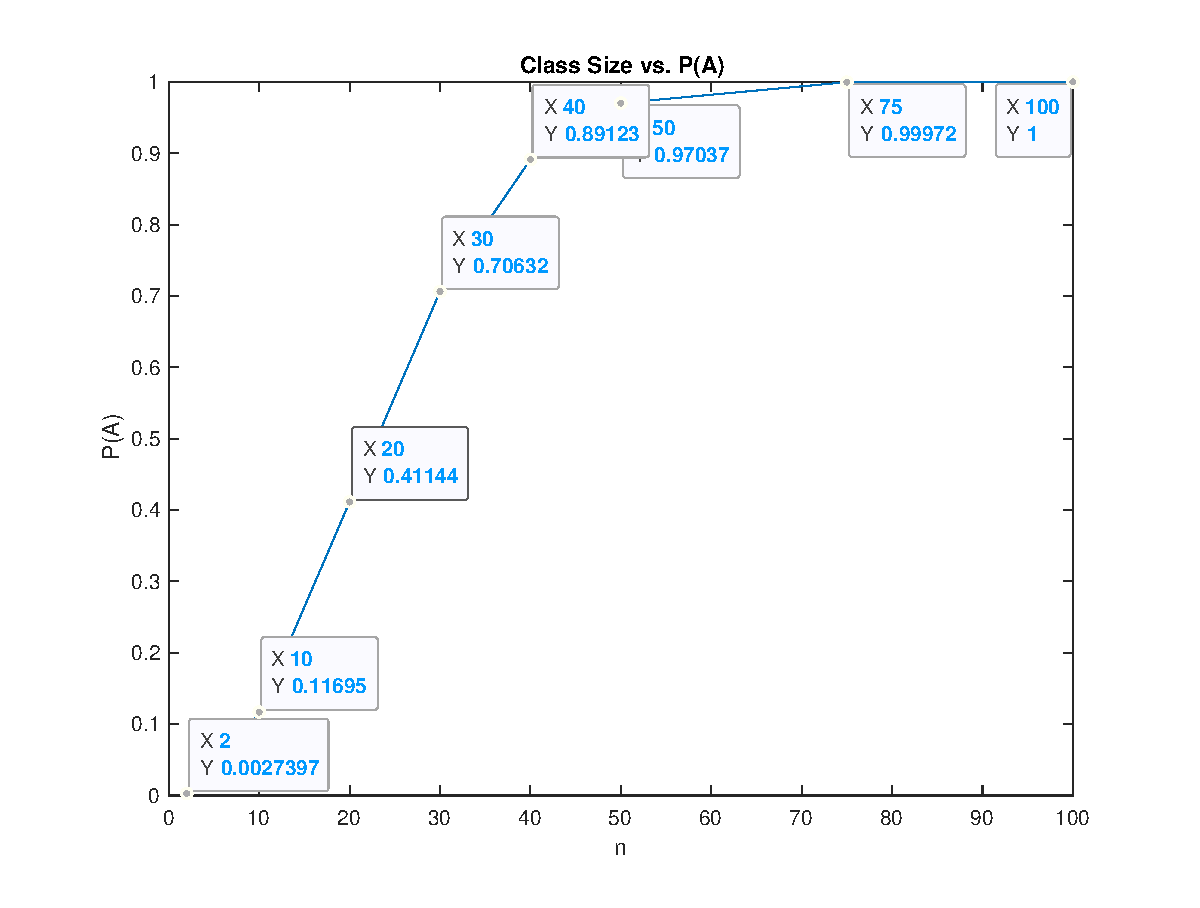
\includegraphics[width=0.8\textwidth]{q1_1}
  \caption{Class Size ($n$) vs. $P(A)$}
  \label{fig:q1}
\end{figure}

\subsection*{Q1.2}
Minimum number of students to make sure that any two students have the same birthday is 366, since there are 365 days in a year.

\section*{Q2}


\subsection*{Q2.1}

$P(S=disease)~=$ 0.011 \\
$P(S=healthy)~=$ 0.989 \\
$P(T=positive|S=disease)~=$ 0.94 \\
$P(T=negative|S=disease)~=$ 0.06 \\
$P(T=positive|S=healthy)~=$ 0.02 \\
$P(T=negative|S=healthy)~=$ 0.98 

\subsection*{Q2.2}

$P(S=disease|T=positive)=\frac{P(T=positive|S=disease) P(S=disease)}{P(T=positive)}=\frac{0.94 \cdot 0.011}{0.94 \cdot 0.011 + 0.02 \cdot 0.989} \approx$ 0.35

Given the test result for a patient is positive, the probability that patient has the disease is 0.35. Therefore it is not reasonable to diagnose a patient with the disease when the test result is positive.

\subsection*{Q2.3}

Since $P(S=disease|T=positive) \neq$ 1, one can \textbf{never} definitely diagnose a patient as sick. That being said, the criterion for \textbf{confidentally} diagnosing a patient as sick is not defined in the question. Given there are $n$ positive test results, the probability that the patient is sick is,

\begin{align} \label{eqn:q2}
P(S=disease|n~positive~tests) &= 1 - 0.65^n
\end{align}

According to equation (\ref{eqn:q2}), if there are seven positive tests, the patient is sick with a probability of $1 - 0.65^7~\approx$ 0.95.

\section*{Q3}

\subsection*{Q3.1}
The test accuracy is $\approx$ \textbf{0.9489}

\subsection*{Q3.2}
Cleavage occurs between the amino acids at the indices below:

(5,~6), (40,~41), (42,~43), (60,~61), (79,~80), (131,~132), (168,~169), (183,~184), (196,~197), (215,~216), (295,~296), (315,~316), (320,~321), (341,~342), (342,~343), (362,~363), (366,~367), (376,~377), (447,~448), (465,~466), (467,~468), (482,~483)

\subsection*{Q3.3}
Normally, these two values should be the same. But I assume the question means the sum of the logarithms by  saying \textbf{``probabilities"}. Thinking that way, one expects that these two values will probably be different since we do not normalize the values while computing them via Bayes rule, and these values actually turn out to be different.

Starting index of the 8-mer assigned to class 1 with highest probability: \textbf{359} \\
Starting index of the 8-mer assigned to class 0 with lowest probability: \textbf{5} 

\subsection*{Q3.4}
In figure (\ref{fig:q4_1}), test accuracy versus alpha is plotted using all the training samples. We see that smoothing does not really improve the performance because we already have an accuracy of 0.9489 without smoothing. The discussion here is, could we have a low test accuracy without smoothing? Yes, because we are using -inf values when we encounter 0 values at theta's. Imagine for some of the test samples, both $P(Y=1|X)$ and $P(Y=0|X)$ is equal to -inf. In this case (equality), we will assign all these samples to class 0, which means we will classify all the samples belonging to class 1 in this set incorrectly. However, in our case, I have checked the test samples and observed that all the test samples that have $P(Y=1|X)$ = -inf belong to class 0, so we do not make incorrect decisions on this test set even though we do not use smoothing. But smoothing may significantly increase the performance with other test sets.

\begin{figure}[h!]
  \centering
  \includegraphics[width=0.8\textwidth]{q4_1}
  \caption{alpha vs. test accuracy using all training samples}
  \label{fig:q4_1}
\end{figure}

In figure (\ref{fig:q4_2}), test accuracy versus alpha is plotted using only first 75 rows of the training samples. We see that smoothing helps in this case increase test accuracy for $alpha~=~1$. This is probably due to the reason discussed in the first part of this question. Smoothing helps us correctly classify the samples belong to class 1 and have $P(Y=0|X)~=~P(Y=1|X)~=~-inf$.

\begin{figure}[h!]
  \centering
  \includegraphics[width=0.8\textwidth]{q4_2}
  \caption{alpha vs. test accuracy using first 75 rows of the training samples}
  \label{fig:q4_2}
\end{figure}

\subsection*{Q3.5}

In figure (\ref{fig:q5}), you can see the test accuracy versus $k$ (\# of features with highest mutual information used). As expected, the test accuracy increases with k, but after some point, it increases very slowly and we can actually see that using only 30-40 features, we can obtain a pretty good test accuracy.

Also, the highest test accuracy is \textbf{0.9527}, which is higher than the one in Q3.1 (\textbf{0.9489}). This is a very small improvement and it may be due to just stochastic processes, but also one should keep that in my that using all the features may lead to overfitting and poor performance in the test set. So this improvement may be due to avoiding overfitting to the training set by using less features.

\begin{figure}[h!]
  \centering
  \includegraphics[width=0.8\textwidth]{q5}
  \caption{k vs. test accuracy}
  \label{fig:q5}
\end{figure}

\subsection*{Q3.6}

In figure (\ref{fig:q6}), you can see proportion of variance explained (PVE) vs. k (\# of principal components used). Also, PVE(3) = \textbf{0.0759}. We can tell by looking at figure (\ref{fig:q6}) and PVE(3) being very small that applying PCA is not really a good idea with this dataset since we can not explain a big portion of variance in the data (like \%90) using a small percentage of features.

\begin{figure}[h!]
  \centering
  \includegraphics[width=0.8\textwidth]{q6}
  \caption{k vs. pve}
  \label{fig:q6}
\end{figure}

\clearpage
\newpage

\section*{Appendix}

\lstset{language=Python}
\lstset{frame=lines}
\lstset{caption={q3main.py}}
\lstset{label={lst:code_direct}}
\lstset{basicstyle=\footnotesize}
\lstinputlisting[language=Python]{q3main.py}


\end{document}
